\documentclass[utf8, draft]{frontiersFPHY} % for Physics and Applied Maths
% \documentclass[utf8]{frontiersFPHY} % for Physics and Applied Maths
\usepackage{graphicx}
\usepackage{amssymb}
\usepackage{siunitx}
\usepackage{amsmath}
\usepackage{soul}
\usepackage{physics}
\usepackage{bm}
\usepackage{subfiles}

\usepackage{url,hyperref,microtype,subcaption}
% \usepackage[onehalfspacing]{setspace}
\usepackage{cleveref}
% \usepackage[font={bold,it}]{caption}

\graphicspath{{../figures/}}

% Define better ref abbreviations
\usepackage{lineno}

% Define some convenience commands
\renewcommand{\d}{\mathrm{d}}
\renewcommand{\k}{\mathrm{K}}
\newcommand{\ca}{\mathrm{Ca}}
\newcommand{\na}{\mathrm{Na}}
\newcommand{\leak}{\mathrm{L}}
\newcommand{\dstar}{d^\star}
\newcommand{\gstar}{g^\star}
\newcommand{\gbar}{\bar g}
\newcommand{\delt}{\Delta t}
\newcommand{\taus}{\tau_s}
\newcommand{\dn}{\delta_n}
\newcommand{\taud}{\tau_d}


\linenumbers


\def\keyFont{\fontsize{8}{11}\helveticabold }
\def\firstAuthorLast{Olenik {et~al.}} %use et al only if is more than 1 author
\def\Authors{Mark Olenik\,$^{1,*}$, and Conor Houghton\,$^{2}$}
% Affiliations should be keyed to the author's name with superscript numbers and be listed as follows: Laboratory, Institute, Department, Organization, City, State abbreviation (USA, Canada, Australia), and Country (without detailed address information such as city zip codes or street names).
% If one of the authors has a change of address, list the new address below the correspondence details using a superscript symbol and use the same symbol to indicate the author in the author list.
\def\Address{$^{1}$School of Biological Sciences, Faculty of Life Sciences, University of Bristol, Bristol, United Kingdom \\
$^{2}$School of Computer Science, Electrical and Electronic Engineering, and Engineering Mathematics, Faculty of Engineering, University of Bristol, Bristol, United Kingdom}
% The Corresponding Author should be marked with an asterisk
% Provide the exact contact address (this time including street name and city zip code) and email of the corresponding author
\def\corrAuthor{Mark Olenik}

\def\corrEmail{m.olenik@bristol.ac.uk}


\begin{document}

\onecolumn
\firstpage{1}


\title[Scalar Poincaré map for bursting]{A scalar Poincaré map for anti-phase bursting in coupled inhibitory neurons with synaptic depression.}


\author[\firstAuthorLast ]{\Authors} %This field will be automatically populated
\address{} %This field will be automatically populated
\correspondance{} %This field will be automatically populated

\extraAuth{}% If there are more than 1 corresponding author, comment this line and uncomment the next one.
%\extraAuth{corresponding Author2 \\ Laboratory X2, Institute X2, Department X2, Organization X2, Street X2, City X2 , State XX2 (only USA, Canada and Australia), Zip Code2, X2 Country X2, email2@uni2.edu}


\maketitle

\begin{abstract}
  \section{}
  Short-term synaptic plasticity is found in many areas of the central nervous system.  In
  the inhibitory half-centre central pattern generators involved in locomotion, synaptic
  depression is believed to act as a burst termination mechanism, allowing networks to
  generate anti-phase bursting patterns of varying periods.  To better understand burst
  generation in these central patter generators, we study a minimal network of two neurons
  coupled through depressing synapses.  Depending on the strength of the synaptic
  conductance between the two neurons, this network can produce symmetric $n-n$ anti-phase
  bursts, where neurons fire $n$ spikes in alternation, with the period of such solutions
  increasing with the strength of the synaptic conductance.  Relying on the timescale
  disparity in the model, we reduce the eight-dimensional network equations to a
  fully-explicit scalar Poincaré burst map.  This map tracks the state of synaptic
  depression from one burst to the next and captures the complex bursting dynamics of the
  network.  Fixed points of this map are associated with stable burst solutions of the
  full network model, and are created through fold bifurcations of maps.  We derive
  conditions that describe period-increment bifurcations between stable $n-n$ and
  $(n+1)-(n+1)$ bursts, producing a full bifurcation diagram of the burst cycle period.
  Predictions of the Poincaré map fit excellently with numerical simulations of the full
  network model and allow the study of parameter sensitivity for rhythm generation.


  \tiny
  \keyFont{ \section{Keywords:} Synaptic depression, Poincaré map, Dynamical system, Neuronal bursting, Central pattern generator}

\end{abstract}

\section{Introduction}
\section{Materials and Methods}
\subfile{sections/methods.tex}

\section{Results}
\subfile{sections/results.tex}

\section{Discussion}
\subfile{sections/discussion.tex}

\section*{Conflict of Interest Statement}
The authors declare that the research was conducted in the absence of any commercial or financial relationships that could be construed as a potential conflict of interest.

\section*{Author Contributions}
MO and CH contributed to conception and design of the study.
MO performed numerical computation and analysis.
All authors contributed to manuscript writing and revision.

\section*{Funding}
This work was supported by the Wellcome Trust Doctoral Training Programme in Neural Dynamics, Grant no. 099699/Z/12/Z.

\section*{Acknowledgements}
The first author thanks the Wellcome Trust for financial support of his Ph.D. study.
We thank Alan Champneys for sharing his insights on non-continuous maps during the course of this research.
We are also grateful to Alan Roberts and Stephen R. Soffe for their comments on earlier versions of the manuscript.

\section*{Data Availability Statement}
The datasets generated for this study are available on request to the corresponding author.

\bibliographystyle{frontiersinHLTH&FPHY} % for Health, Physics and Mathematics articles
\bibliography{bibliography.bib}

\section*{Figure captions}

\begin{figure}[h!]
  \centering
  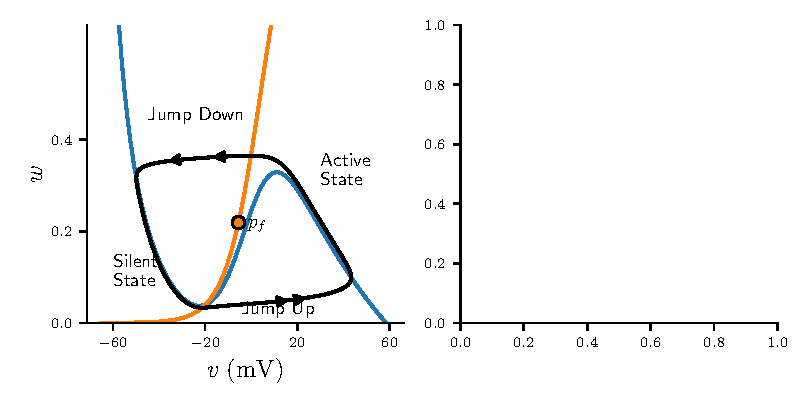
\includegraphics{fig/nullclines-uncoupled.pdf}
  \caption{Periodic solution of relaxation-oscillator model neuron. $\bm{\mathrm{(A)}}$ Projection of limit cycle onto ($v,w$)-phase plane with $v$-nullcline (blue, $v_\infty$) and $w$-nullcline (orange, $w_\infty$). Unstable fixed point $p_{f}$ is indicated by an orange dot. $\bm{\mathrm{(B)}}$ Corresponding voltage trace $v(t)$ of an action potential.~\label{fig:nullclines}}
\end{figure}

\begin{figure}[h!]
  \centering
  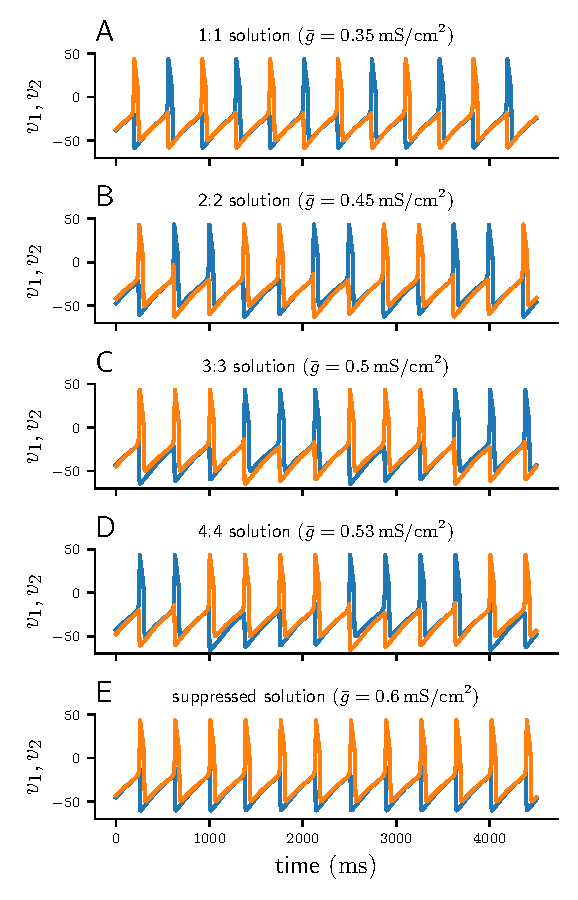
\includegraphics{fig/depression-traces.pdf}
  \caption{Solution profiles of a $4-4$ burst. $\bm{\mathrm{(A)}}$ Membrane potentials of cell 1 ($v_{1}$, blue), and cell 2 ($v_{2}$, orange). $\bm{\mathrm{(B)}}$ Synaptic variables $d_{1}$ (blue) and $s_{1}$ (grey) of cell 1.~\label{fig:depression-traces}}
\end{figure}

\begin{figure}[h!]
  \centering
  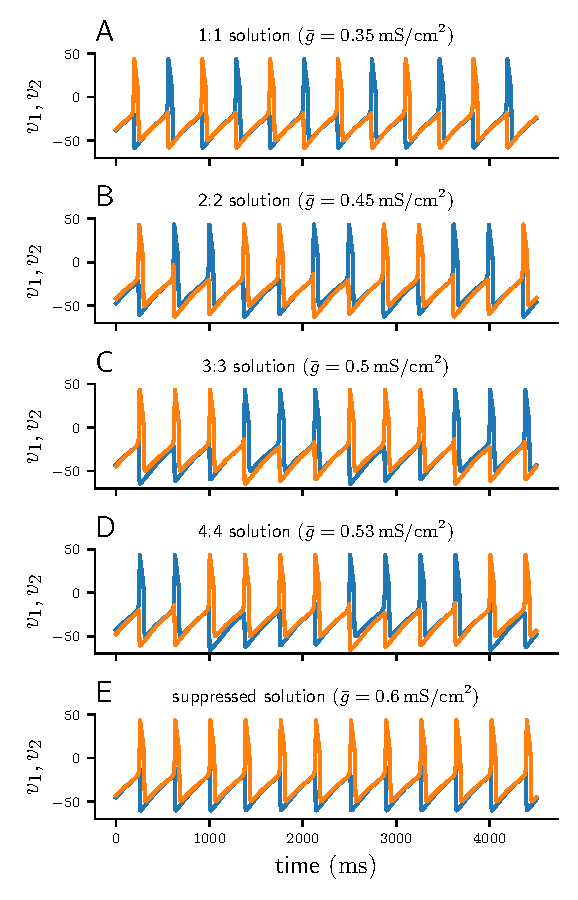
\includegraphics{fig/burst-sols.pdf}
  \caption{Voltage traces of both cells of numerically stable solutions for increasing values of the coupling strength $\gbar$ (increasing top to bottom).~\label{fig:burst-sols}}
\end{figure}

\begin{figure}[h!]
  \centering
  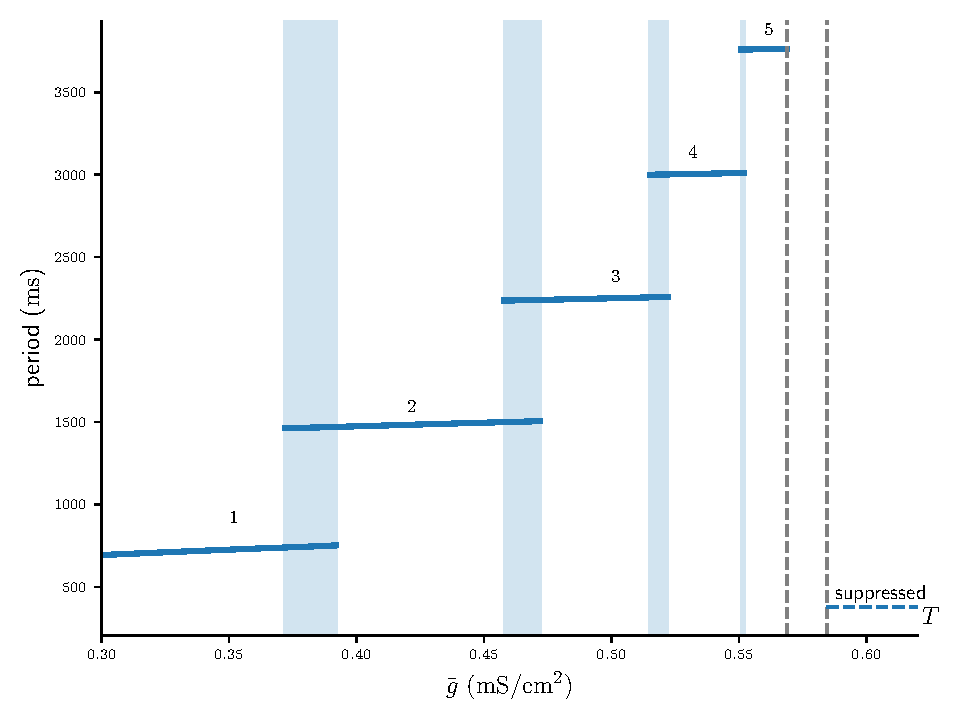
\includegraphics{fig/bif-diagram.pdf}
  \caption{Numerically computed bifurcation diagrams of stable $n-n$ solutions for increasing coupling strength $\gbar$. $\bm{\mathrm{(A)}}$ Period of stable solutions. Dashed lines show the interval between the $5-5$ and the suppressed solutions, where higher period $n-n$ solutions occur on increasingly smaller intervals of $\gbar$. $\bm{\mathrm{(B)}}$ $ISI$s corresponding to $n-n$ solutions in $\mathrm{(A)}$. Long $ISI$s are associated with the quiet phase of a burst, short $ISI$s with the free phase. During the free phase, $ISI$s are of approximately constant duration $T$.\label{fig:bif-diagram}}
\end{figure}

\begin{figure}[h!]
  \centering
  \includegraphics{fig/nullclines-coupled.pdf}
  \caption{Nullclines $v_{\infty}$ (blue) and $w_{\infty}$ (orange) in the $(v,w$)-phase plane for different values of the total synaptic conductance $\gbar s$. For small $\gbar s < g^{\star}$, fixed point $p_{f}$ is unstable (orange point). Larger values $\gbar s$ move $v_{\infty}$ down in the $(v,w)$-plane until $p_{f}$ changes stability (half orange,  half blue point) at some critical total conductance value $\gbar s = g^{\star}$, and becomes stable (blue point) for $\gbar>g^{\star}$.~\label{fig:nullclines-coupled}}
\end{figure}

\begin{figure}[h!]
  \centering
  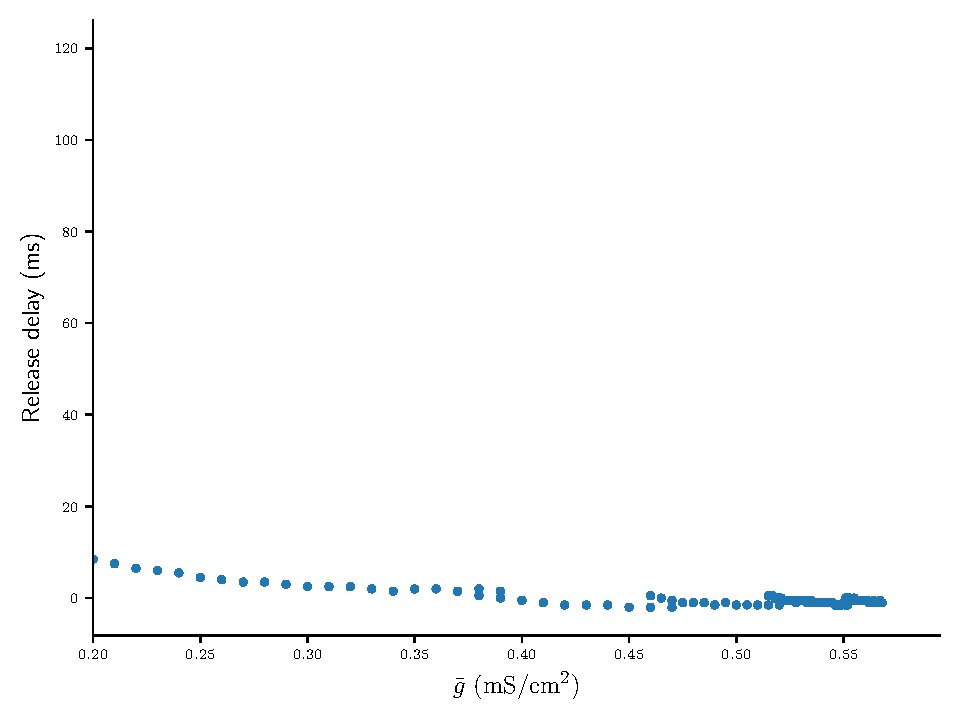
\includegraphics[width=0.8\textwidth]{fig/release-delay.pdf}
  \caption{Numerically computed values of the release delay for varying $\gbar$. Each of the three branches (A, B, C) also shows the timecourse of the total synaptic conductance $\gbar s$ of a sample stable solution of both cells (blue and orange), as well as the release conductance $g^{\star}$ (dashed green line). $\bm{\mathrm{(A)}}$ Branch corresponding to the $1-1$ solution. Here the quiet cell only spikes after a significant release delay. $\bm{\mathrm{(B)}}$ Branch with a long release delay associated with a subset of $2-2$ solutions. Here the release condition is briefly satisfied after the first spike of cell 1. This does not cause firing of cell 2, which only occurs after the second spike of cell 1. $\bm{\mathrm{(C)}}$ Branch with $n-n$ solutions  where release delay is approximately zero and the release condition is sufficient for firing of cell 2.
    ~\label{fig:release-delay}}
\end{figure}

\begin{figure}[h!]
  \centering
  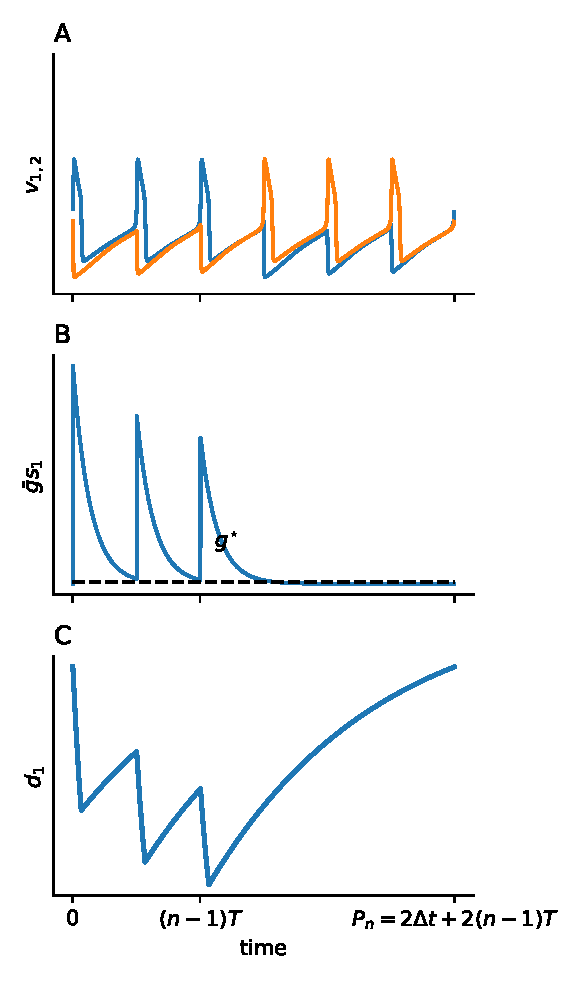
\includegraphics{fig/free-quiet.pdf}
  \caption{Schematic diagram of the free and quiet phases for a $3-3$ solution. $\bm{\mathrm{(A)}}$ Membrane potentials of cell 1 ($v_{1}$) and cell 2 ($v_{2}$).  The grey patches depict inter-burst-intervals $\delt$. $\bm{\mathrm{(B)}}$ Total synaptic conductance of cell 1 ($\gbar s_1$) as it crosses the release conductance $g^{\star}$. $\bm{\mathrm{(C)}}$ Solution $d_1(t)$ of depression variable of cell 1, during free (blue) and quiet phases (orange).~\label{fig:free-quiet1}}
\end{figure}

\begin{figure}[h!]
  \centering
  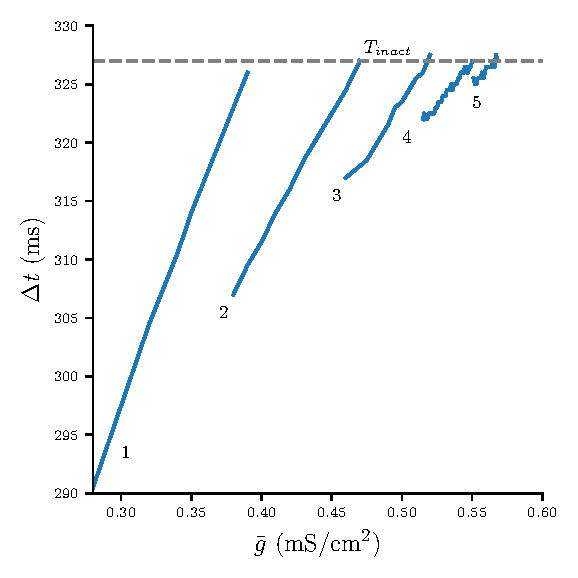
\includegraphics{fig/delta-t.pdf}
  \caption{Numerically computed bifurcation diagram of $\delt$ for varying $\gbar$. Each continuous branch is associated with a stable $n-n$ burst solution. Increasing $\gbar$ increases $\Delta t$ until the solutions bifurcate at $\Delta t\approx T$.~\label{fig:delta-t}}
\end{figure}

\begin{figure}[h!]
  \centering
  \includegraphics{fig/FQ-map.pdf}
  \caption{Maps $F_n$ $\bm{\mathrm{(A)}}$ and $Q_n$ $\bm{\mathrm{(B)}}$ for $\gbar=0.6$ $\si{mS/cm^{2}}$ and $n=1,2,3,4$. Curves $F_n$ intersect at $d_{s}$ which is indicated by a dashed vertical line.~\label{fig:FQ-map}}
\end{figure}

\begin{figure}[h!]
  \centering
  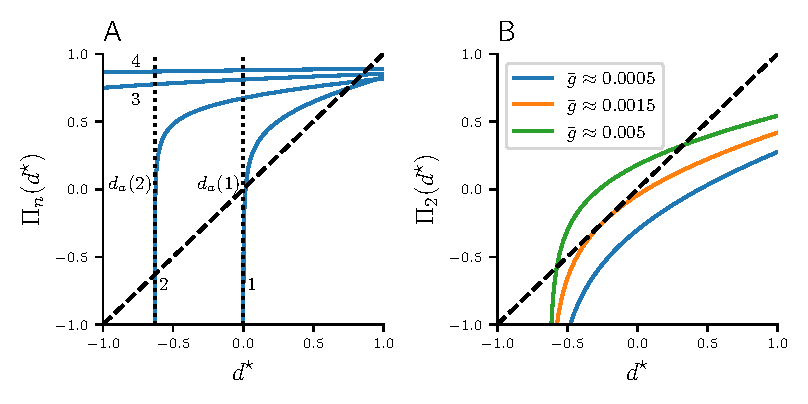
\includegraphics{fig/Pn-map.pdf}
  \caption{Map $\Pi_{n}:d^{\star}$. $\bm{\mathrm{(A)}}$ $\Pi_{n}$ for $n=1,2,3,4$ at $\gbar=0.6$ $\si{mS/cm^{2}}$. $\bm{\mathrm{(B)}}$ $\Pi_{2}$ with $n=2$ for varying $\gbar \approx 0.01, 0.034, 0.3$ $\si{mS/cm^{2}}$. The identity function is illustrated by a diagonal line.~\label{fig:Pn-map}}
\end{figure}

\begin{figure}[h!]
  \centering
  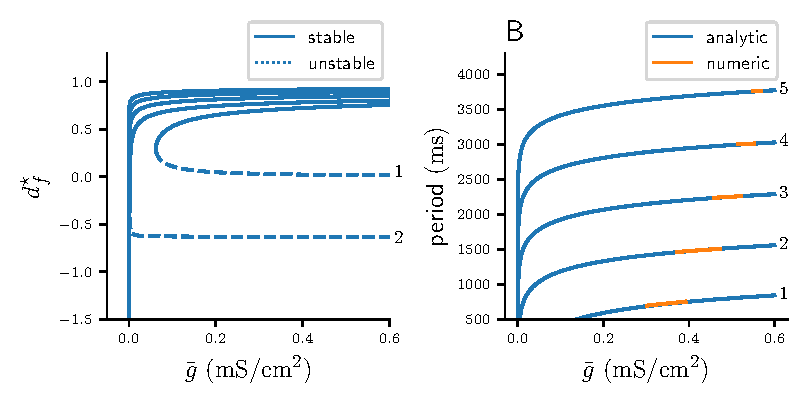
\includegraphics{fig/folds.pdf}
  \caption{$\bm{\mathrm{(A)}}$ Fold bifurcation diagrams of stable (continuous curves) and unstable (dotted curves) fixed points of $\Pi_{n}$ for varying $n$. $\bm{\mathrm{(B)}}$ Cycle periods computed from stable fixed points (blue), and the corresponding solution period from numerical integration of the system of ODEs (orange).~\label{fig:folds}}
\end{figure}

\begin{figure}[h!]
  \centering
  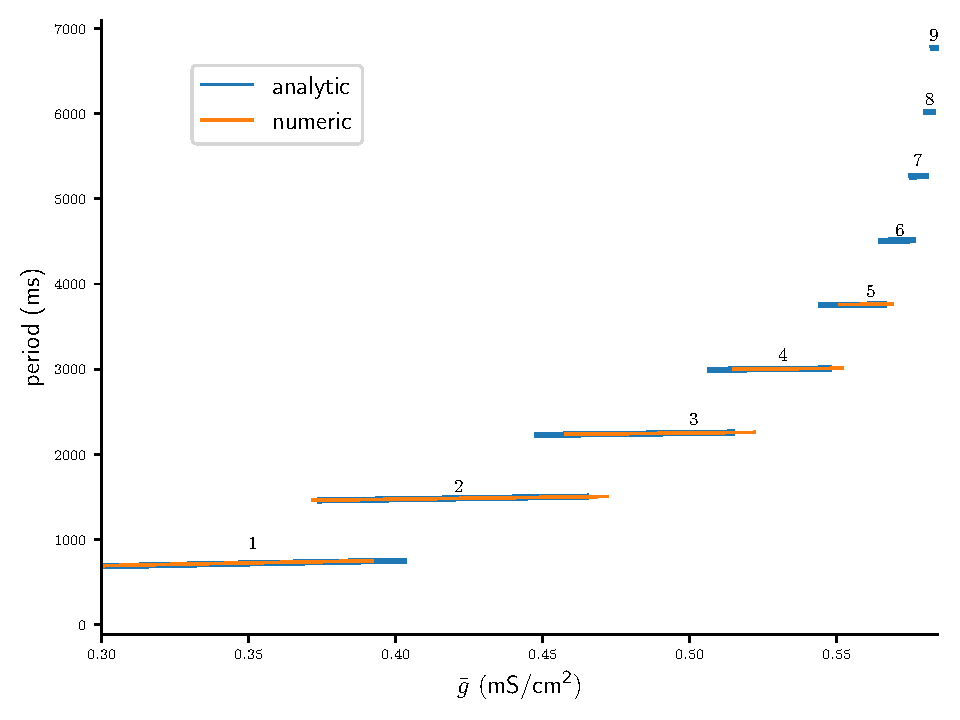
\includegraphics[width=0.8\textwidth]{fig/final-bif.pdf}
  \caption{Bifurcation diagrams of stable $n-n$ solutions computed analytically from fixed points of $\Pi_n$ and plotted on the respective intervals of $\gbar\in \big[\gbar_+(n),\gbar_-(n)\big]$ (blue), and computed from numerical integrations of the ODEs (orange).~\label{fig:final-bif}}
\end{figure}

\end{document}
